\documentclass{beamer} 
\usetheme{default} 
\usecolortheme{albatross}
\setbeamercovered{transparent}
%\useoutertheme{umbcfootline}  


\usepackage[spanish]{babel}
%\usepackage[latin1]{inputenc}
\usepackage[utf8x]{inputenc}
\usepackage{hyperref}
\usepackage{color}



\usepackage{multicol}



\title{Entrada y Salida}

\author{Manuel J. Molino Milla \and Luis Molina Garzón}

\date{\today} %

\institute{IES Virgen del Carmen \and Departamento de Informática}




%\beamerdefaultoverlayspecification{<+->}

\begin{document}


\begin{frame}
  \titlepage
\end{frame}

\begin{frame}
    \frametitle{Logo}
\begin{figure}

\includegraphics[scale=1]{imagenes/logo.jpeg} 
\caption{Logo Java}
\end{figure}
\end{frame}

\begin{frame}
  \frametitle{Contenido}
  \tableofcontents[pausesections]
\end{frame}

\section{Clase File}
\begin{frame}
\frametitle{Clase File}
\begin{itemize}[<+-|alert@+>]
\item El almacenamiento en arrays, variables o colecciones es temporal.
\item Se pierden cuando el programa termina.
\item Podemos almecenar los datos en un fichero.
\item Hablamos de \alert{persistencia de datos}
\item El nombre del fichero puede indicarse de forma absoluta o relativa.
\item \emph{c:$\backslash$book$\backslash$Welcome.java} o \emph{/home/usuario/book/Welcome.java}
\item \emph{.$\backslash$Welcome.java} o \emph{./Welcome.java}
\end{itemize}
\pause
\end{frame}


\begin{frame}[fragile]
\frametitle{Clase File}
\framesubtitle{¿Qué hace cada método?}
\begin{figure}
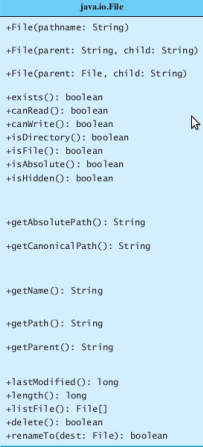
\includegraphics[scale=0.65]{imagenes/file.png}
\end{figure}
\end{frame}

\begin{frame}[fragile]
\frametitle{Ejemplo}
\begin{scriptsize}
\begin{verbatim}
public class TestFileClass {
  public static void main(String[] args) {
  java.io.File file = new java.io.File("./fichero.txt");
  System.out.println("¿Existe fichero? " + file.exists() );
  System.out.println("El fichero tiene " + file.length() + " bytes");
  System.out.println("¿Es de lectura? " + file.canRead());
  System.out.println("¿Es de escritura? " + file.canWrite());
  System.out.println("¿Es un directoio? " + file.isDirectory());
  System.out.println("¿Es un fichero? " + file.isFile());
  System.out.println("¿Está oculto? " + file.isHidden());
  System.out.println("paht absoluto es " + file.getAbsolutePath());
  System.out.println("Última modificación " + new
                             java.util.Date(file.lastModified()));
\end{verbatim}
\end{scriptsize}
\end{frame}

\section{Clase PrintWriter}
\begin{frame}
\frametitle{Clase PrintWriter}
\framesubtitle{Crea y permite escribir datos a un fichero de texto}
\pause
\begin{multicols}{2}
\begin{figure}
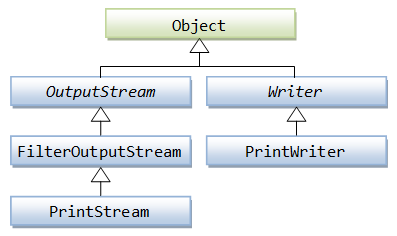
\includegraphics[scale=0.55]{imagenes/pw.png} 
\caption{UML de la clase PrintWriter}
\end{figure} 
\begin{small}
\begin{enumerate}[<+-| alert@+>]
      \item Crea objeto \emph{PrintWriter} para el objeto \emph{File}
      \item Crea un objeto \emph{PrintWriter} especificado el nombre del fichero.
      \item Escribe un string al fichero.
      \item Escribe un char al fichero.
      \item Escribe un array de char al fichero.
      \item Escribe un int, long, float, double o boolean al fichero..
      \end{enumerate}
\end{small}
\end{multicols}
\pause
  
\end{frame}


\begin{frame}[fragile]
\frametitle{Ejemplo}
\begin{small}
\begin{verbatim}
public class WriteData {
  public static void main(String[] args) throws Exception {
   java.io.File file = new java.io.File("nuevo.txt");
   if (file.exists()) {
    System.out.println("El fichero ya existe");
    System.exit(0);
   }
// Crea un fichero
   java.io.PrintWriter output = new java.io.PrintWriter(file);
//Escribe en el fichero
   output.print("John T Smith ");
   output.println(90);
   output.print("Eric K Jones ");
   output.println(85);
// Cerramos el fichero
   output.close();
  }
}
\end{verbatim}
\end{small}
\end{frame}

\section{Clase Scanner}
\begin{frame}
\frametitle{Clase Scanner}

\begin{multicols}{2}
\begin{figure}
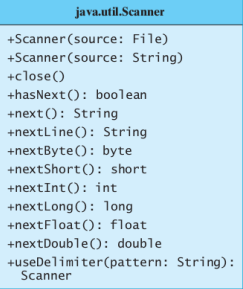
\includegraphics[scale=0.55]{imagenes/scanner.png} 
\caption{UML de la clase Scanner}
\end{figure} 
\begin{small}
\begin{enumerate}[<+-| alert@+>]
      \item Crea un scanner que produce el valor escaneado desde un fichero.
      \item Crea un scanner que produce el valor escaneado desde un string.
      \item Cierra el scanner.
      \item Devuelve true si el scanner tiene mas datos que leer.
      \item Devuelve el siguiente token como un string desde el scanner.
      \item Devuelve el siguiente token como un byte, short, int, long, float, doublestring desde el scanner.
      \item Configura el scanner con un patrón delimitador y devuelve el scanner.
      \end{enumerate}
\end{small}
\end{multicols}  
\pause
\end{frame}

\begin{frame}[fragile]
\frametitle{Ejemplo}
\begin{small}
\begin{verbatim}
import java.util.Scanner;
public class ReadData {
  public static void main(String[] args) throws Exception {
// Create un objeto File 
  java.io.File file = new java.io.File("nuevo.txt");
// Crea el Scanner para el fichero
  Scanner input = new Scanner(file);
// Lee datos desde el fichero nuevo.txt
  while (input.hasNext()) {
    String firstName = input.next();
    String n = input.next();
    String lastName = input.next();
    int score = input.nextInt();
    System.out.println(
    firstName + " " + n + " " + lastName + " " + score);
  }
// Close the file
  input.close();
 }
}
\end{verbatim}
\end{small}
\end{frame}

\begin{frame}
\frametitle{Preguntas} 
\begin{figure}

\includegraphics[scale=0.9]{imagenes/dudas.png} 
\end{figure} 
\end{frame}

\end{document}

